\documentclass[conference]{IEEEtran}
\usepackage[utf8]{inputenc}
\usepackage[spanish, es-tabla]{babel}
\usepackage{graphicx}
\graphicspath{{./imagenes/}{./}}
\DeclareGraphicsExtensions{.pdf,.jpeg,.png}
\usepackage{amsmath, amssymb, amsfonts}
\usepackage{siunitx}
\usepackage{xcolor}
\usepackage{booktabs}
\usepackage{hyperref}
\usepackage{listings}
\usepackage{tikz}
\usetikzlibrary{babel, arrows.meta, positioning, shapes.geometric, decorations.pathreplacing, calc, backgrounds, fit}

% Configuracion estetica para listados de codigo y tramas JSON
\lstset{
    backgroundcolor=\color{black!4},
    basicstyle=\ttfamily\scriptsize,
    frame=single,
    framerule=0.5pt,
    rulecolor=\color{black!30},
    breaklines=true,
    captionpos=b,
    abovecaptionskip=6pt,
    belowcaptionskip=6pt,
    showstringspaces=false
}

\begin{document}

\title{Sistema de Monitoreo IoT vía Web sobre Dirección IP Pública: \\ Arquitectura Telemática, Despliegue en la Nube y Procesamiento en Tiempo Real}

\author{
    \IEEEauthorblockN{Diomar Castro y Miguel Ángel Rodríguez}
    \IEEEauthorblockA{
        \textit{Facultad de Ciencias Básicas e Ingeniería, Universidad de los Llanos} \\
        \textit{Villavicencio, Meta, Colombia} \\
        {\small \texttt{diomar.castro@unillanos.edu.co} \quad Código: 161004708}\\
        {\small \texttt{marodriguez.payares@unillanos.edu.co} \quad Código: 161004834}
    }
}

\maketitle

\begin{abstract}
El presente artículo expone el diseño, despliegue y validación experimental de un sistema telemático integral para el monitoreo en tiempo real de variables termodinámicas y radioeléctricas (Temperatura, Humedad Relativa, Índice de Calor, Punto de Rocío y Potencia de Señal RSSI), transmitidas por un nodo sensor físico ESP32 hacia un Servidor Virtual en la Nube con Dirección IP Pública enrutada en Internet. La solución supera las restricciones de confinamiento en redes privadas (NAT/LAN) mediante la implementación de una arquitectura cliente-servidor robusta basada en el protocolo HTTP/1.1 con serialización JSON, un proxy inverso Nginx con mitigación de buffering, un servidor de aplicaciones Flask concurrente con persistencia SQLite y un canal de empuje continuo unidireccional fundamentado en Server-Sent Events (SSE). Asimismo, se diseñó un algoritmo de suavizado gaussiano discreto simétrico de 5 puntos en el cliente para atenuar el ruido de cuantización inherente a los sensores digitales, desplegando un dashboard web ultra-minimalista, responsivo en terminales móviles y protegido bajo protocolos TLS/HTTPS. Los resultados experimentales confirman una latencia media de transporte inferior a 85 ms y una disponibilidad operativa del 100\% bajo pruebas de estrés.
\end{abstract}

\begin{IEEEkeywords}
Internet de las Cosas (IoT), Dirección IP Pública, ESP32, Server-Sent Events (SSE), Nginx, Regresión de Rothfusz, Filtro Gaussiano, Telemetría en Tiempo Real.
\end{IEEEkeywords}

\section{Introducción}
El despliegue de redes de sensores en el Internet de las Cosas (\textit{Internet of Things}, IoT) enfrenta comúnmente el confinamiento de dispositivos dentro de redes de área local (LAN) aisladas tras pasarelas de traducción de direcciones de red (\textit{Network Address Translation}, NAT) \cite{tanenbaum2021}. Cuando un nodo embebido debe reportar variables hacia una plataforma accesible globalmente, la carencia de una dirección IP pública enrutable obliga al uso de túneles VPN o servidores intermediarios con penalizaciones de latencia y sobrecostos operativos \cite{kurose2017}.

Para resolver esta limitación, este trabajo presenta el diseño, despliegue y validación de un sistema telemático integral para la asignatura \textit{Sistemas de Comunicación II} (Semestre 2026-II), orientado a cumplir los siguientes objetivos de ingeniería:
\begin{enumerate}
    \item Despliegue de un Servidor Virtual en la Nube (VPS) con asignación de dirección IPv4 pública estática en Internet.
    \item Puesta en producción de la pila de servicios web perimetral y de aplicación (Nginx, Gunicorn, Flask y SQLite).
    \item Ejecución continua y no bloqueante del servicio de ingesta telemática.
    \item Conexión y transmisión autónoma de variables ambientales desde un nodo físico ESP32 con sensor DHT22 bajo TCP/IP.
    \item Visualización reactiva en tiempo real mediante empuje de eventos en el servidor (\textit{Server-Sent Events}), eliminando el sondeo periódico.
\end{enumerate}

\section{Marco Teórico y Fundamentos Telemáticos}

\subsection{Modelo de Capas y Pila de Protocolos IoT}
La transmisión de datos se fundamenta en la arquitectura de cuatro capas del modelo TCP/IP, adaptada a nodos de cómputo embebido de bajo consumo:

\begin{enumerate}
    \item \textbf{Capa de Enlace y Física (IEEE 802.11 b/g/n):} El ESP32 modula la información en la banda ISM de \SI{2.4}{\giga\hertz} mediante multiplexación por división de frecuencias ortogonales (OFDM). La calidad del enlace radioeléctrico se cuantifica a través del Indicador de Fuerza de Señal Recibida (\textit{Received Signal Strength Indicator}, RSSI), modelado en decibelios-milivatio (\si{\decibel m}) mediante el modelo log-distancia:
    \begin{equation}
        \text{RSSI}(d) = \text{RSSI}(d_0) - 10 n \log_{10}\left(\frac{d}{d_0}\right) + X_\sigma
        \label{eq:rssi}
    \end{equation}
    donde $d$ es la distancia al punto de acceso, $n$ es el exponente de pérdidas de trayectoria y $X_\sigma$ representa el desvanecimiento por sombreado (\textit{shadowing}) gaussiano \cite{forouzan2013}.
    
    \item \textbf{Capa de Red (IPv4):} El datagrama IP se transporta directamente hacia la dirección IPv4 pública estática del servidor (\texttt{57.156.57.129}), superando el aislamiento impuesto por NAT (RFC 1918).
    
    \item \textbf{Capa de Transporte (TCP, RFC 793):} Se emplea TCP para garantizar entrega ordenada, libre de duplicados y con control de congestión ante pérdidas en el canal \cite{rfc793}.
    
    \item \textbf{Capa de Aplicación (HTTP/1.1 y JSON):} Las mediciones se serializan en tramas JSON y se despachan mediante el endpoint \texttt{POST /api/readings} con cabecera \texttt{application/json} \cite{rfc7230, rfc8259}.
\end{enumerate}

\subsection{Transmisión Push en Tiempo Real: Server-Sent Events (SSE)}
Frente al sondeo periódico (\textit{polling}), cuya sobrecarga de cabeceras HTTP escala como $O(N)$ peticiones concurrentes, el sistema implementa la especificación W3C \textit{Server-Sent Events} (SSE) sobre \texttt{/api/stream}. El cliente establece una conexión persistente (\texttt{Accept: text/event-stream}) y el servidor empuja asíncronamente las lecturas entrantes (\autoref{lst:sse}):
\begin{lstlisting}[caption={Estructura de transmisión SSE emitida hacia los clientes web.}, label={lst:sse}]
event: new_reading
data: {"temperature": 24.3, "humidity": 61.2, "status": "NORMAL", ...}
\end{lstlisting}
Este esquema unidireccional abate la latencia de entrega a escala de milisegundos y suprime el tráfico redundante.

\subsection{Modelado de Variables Termodinámicas Derivadas}
El servidor en la nube no se limita al almacenamiento pasivo, sino que evalúa balances psicrométricos en tiempo real:

\subsubsection{\texorpdfstring{Índice de Calor / Sensación Térmica ($HI$)}{Índice de Calor (HI)}}
Se evalúa mediante la formulación multivariante de regresión de Rothfusz (NOAA) \cite{rothfusz1990}. A partir de la temperatura en grados Fahrenheit ($T_F$) y la humedad relativa ($R \in [0, 100]$):
\begin{align}
    HI_F = &-42.379 + 2.04901523\,T_F + 10.14333127\,R \nonumber \\
           &- 0.22475541\,T_F R - 0.00683783\,T_F^2 \nonumber \\
           &- 0.05481717\,R^2 + 0.00122874\,T_F^2 R \nonumber \\
           &+ 0.00085282\,T_F R^2 - 0.00000199\,T_F^2 R^2
    \label{eq:heat_index}
\end{align}
El valor resultante se normaliza a escala Celsius mediante $HI_{\si{\celsius}} = (HI_F - 32) \cdot \frac{5}{9}$.

\subsubsection{\texorpdfstring{Punto de Rocío ($T_d$)}{Punto de Rocío (Td)}}
Representa la temperatura de condensación del vapor de agua a presión constante. Se calcula mediante la formulación de Magnus-Tetens \cite{alduchov1996}:
\begin{equation}
    \alpha = \frac{a \cdot T}{b + T} + \ln\left(\frac{RH}{100}\right), \quad T_d = \frac{b \cdot \alpha}{a - \alpha}
    \label{eq:dew_point}
\end{equation}
con parámetros empíricos $a = 17.27$ y $b = \SI{237.7}{\celsius}$.

\subsection{Filtrado Gaussiano de Señales de Telemetría}
La cuantización finita del DHT22 ($\Delta T = \SI{0.1}{\celsius}$, $\Delta RH = \SI{1}{\percent}$) induce fluctuaciones en diente de sierra en escalas gráficas estrechas. Para garantizar una curva continua sin enmascarar la dinámica real, se aplicó un filtro de respuesta al impulso finita (FIR) simétrico de ponderación gaussiana \cite{oppenheim1999}:
\begin{equation}
    y[n] = \frac{1}{\sum_{k=-M}^{M} w_k} \sum_{k=-M}^{M} w_k \, x[n+k]
    \label{eq:gauss_filter}
\end{equation}
con ventana de 5 puntos ($M=2$), vector de ponderación $\mathbf{w} = [1, \, 3, \, 5, \, 3, \, 1]$ y suma $\sum w_k = 13$. Asimismo, se fijó un margen lineal del 12\% (\textit{grace}) en Chart.js para evitar la sobrerepresentación de microvariaciones.

% FIGURA TIKZ 1: ARQUITECTURA GENERAL DEL SISTEMA
\begin{figure*}[t]
\centering
\begin{tikzpicture}[
    >=Latex, thick,
    block/.style={draw, rounded corners=3pt, fill=blue!6, minimum width=2.4cm, minimum height=1.1cm, align=center, font=\footnotesize},
    cloudblock/.style={draw, rounded corners=6pt, fill=orange!8, minimum width=2.5cm, minimum height=1.1cm, align=center, font=\footnotesize},
    clientblock/.style={draw, rounded corners=3pt, fill=green!8, minimum width=2.4cm, minimum height=1.1cm, align=center, font=\footnotesize},
    arrowlabel/.style={font=\scriptsize, align=center}
]

    % Bloque 1: Entorno y Sensor
    \node[block] (sensor) {\textbf{Entorno Físico}\\\scriptsize Sensor DHT22\\\scriptsize(Temp y Humedad)};
    
    % Bloque 2: ESP32
    \node[block, right=0.8cm of sensor] (esp32) {\textbf{Nodo ESP32}\\\scriptsize GPIO 4 / Conversión\\\scriptsize Pila Wi-Fi IEEE 802.11};
    
    % Bloque 3: Internet / IP Publica
    \node[cloudblock, right=0.9cm of esp32] (wan) {\textbf{Red WAN / Internet}\\\scriptsize Dirección IPv4 Pública\\\texttt{57.156.57.129:80}};
    
    % Bloque 4: Nginx + Gunicorn
    \node[cloudblock, right=0.9cm of wan] (vps) {\textbf{Servidor Cloud (VPS)}\\\scriptsize Nginx (Proxy Inverso)\\\scriptsize Gunicorn + Flask WSGI};
    
    % Bloque 5: SQLite
    \node[block, fill=purple!8, above=0.7cm of vps] (db) {\textbf{Base de Datos}\\\scriptsize SQLite3\\\texttt{data/telemetry.db}};
    
    % Bloque 6: Cliente Web
    \node[clientblock, right=0.9cm of vps] (client) {\textbf{Navegador Web}\\\scriptsize Dashboard Minimalista\\\scriptsize Chart.js + SSE};

    % Conexiones
    \draw[->] (sensor) -- node[above, arrowlabel] {1-Wire\\(GPIO 4)} (esp32);
    \draw[->] (esp32) -- node[above, arrowlabel] {Wi-Fi Link\\POST JSON} (wan);
    \draw[->] (wan) -- node[above, arrowlabel] {TCP Port 80\\Inbound} (vps);
    \draw[<->] (vps) -- node[right, arrowlabel] {Lectura /\\Escritura} (db);
    \draw[->] (vps) -- node[above, arrowlabel] {Push SSE\\Stream} (client);

\end{tikzpicture}
\caption{Arquitectura telemática integral del sistema de monitoreo IoT sobre dirección IP pública.}
\label{fig:arquitectura_sistema}
\end{figure*}

\section{Metodología y Diseño de Ingeniería}

\subsection{Etapa 1: Acondicionamiento del Hardware Sensor (ESP32)}
El circuito de captura física está constituido por un microcontrolador ESP32-WROOM-32 y un transductor digital de humedad y temperatura DHT22 (AM2302) \cite{dht22manual}. Las interconexiones se detallan en la \autoref{tab:hardware_pinout}:

\begin{table}[htbp]
\centering
\caption{Asignación de terminales físicos del hardware IoT.}
\label{tab:hardware_pinout}
\resizebox{\columnwidth}{!}{%
\begin{tabular}{lll}
\toprule
\textbf{Pin DHT22} & \textbf{Pin ESP32} & \textbf{Función y Acondicionamiento} \\
\midrule
Pin 1 (VCC)  & 3V3 (3.3V DC) & Alimentación regulada de bajo ruido \\
Pin 2 (DATA) & GPIO 4 (D4)   & Bus 1-Wire bidireccional con pull-up \SI{10}{\kilo\ohm} \\
Pin 3 (NC)   & Sin conexión  & Desconectado internamente \\
Pin 4 (GND)  & GND           & Retorno de masa de señal común \\
\bottomrule
\end{tabular}%
}
\end{table}

El firmware en Arduino C++ opera mediante un temporizador no bloqueante basado en \texttt{millis()}, evitando bloqueos (\texttt{delay()}) en la conectividad Wi-Fi. Cada \SI{5000}{\milli\second}, el nodo muestrea las variables, adquiere el RSSI y despacha la trama al servidor mediante \texttt{HTTPClient}.

% FIGURA TIKZ 2: DIAGRAMA DE SECUENCIA DE PROTOCOLOS
\begin{figure}[htbp]
\centering
\begin{tikzpicture}[>=Latex, thick, font=\scriptsize]
    % Lineas verticales
    \node (esp) at (0, 0) [draw, fill=blue!10, rounded corners=2pt, minimum width=1.5cm] {ESP32};
    \node (srv) at (3.2, 0) [draw, fill=orange!10, rounded corners=2pt, minimum width=1.5cm] {Nginx / Flask};
    \node (cli) at (6.4, 0) [draw, fill=green!10, rounded corners=2pt, minimum width=1.5cm] {Cliente Web};
    
    \draw[dashed, gray] (esp.south) -- ++(0, -5.2);
    \draw[dashed, gray] (srv.south) -- ++(0, -5.2);
    \draw[dashed, gray] (cli.south) -- ++(0, -5.2);
    
    % Conexión SSE del cliente
    \draw[->, green!60!black] ([yshift=-0.6cm]cli.south) -- node[above, sloped] {GET /api/stream (SSE)} ([yshift=-1.0cm]srv.south);
    \draw[->, dashed, green!60!black] ([yshift=-1.2cm]srv.south) -- node[above, sloped] {200 OK (Keep-Alive)} ([yshift=-1.6cm]cli.south);
    
    % Handshake TCP ESP32
    \draw[->, blue!70!black] ([yshift=-2.0cm]esp.south) -- node[above, sloped] {TCP SYN [Port 80]} ([yshift=-2.3cm]srv.south);
    \draw[<-, blue!70!black] ([yshift=-2.6cm]esp.south) -- node[above, sloped] {TCP SYN-ACK} ([yshift=-2.3cm]srv.south);
    \draw[->, blue!70!black] ([yshift=-2.9cm]esp.south) -- node[above, sloped] {TCP ACK} ([yshift=-3.2cm]srv.south);
    
    % Transmision HTTP POST
    \draw[->, black, very thick] ([yshift=-3.5cm]esp.south) -- node[above, sloped] {\textbf{POST} /api/readings (JSON)} ([yshift=-3.8cm]srv.south);
    \draw[<-, black] ([yshift=-4.2cm]esp.south) -- node[above, sloped] {HTTP 201 Created} ([yshift=-3.9cm]srv.south);
    
    % Push SSE al cliente
    \draw[->, purple!80!black, very thick] ([yshift=-4.3cm]srv.south) -- node[above, sloped] {\textbf{Push SSE}: event: new\_reading} ([yshift=-4.7cm]cli.south);

\end{tikzpicture}
\caption{Diagrama de secuencia temporal de la transacción telemática.}
\label{fig:diagrama_secuencia}
\end{figure}

\subsection{Etapa 2: Aprovisionamiento en Microsoft Azure (IaaS)}
Se desplegó una máquina virtual en Microsoft Azure conforme a los requerimientos del proyecto (\autoref{tab:azure_specs}):

\begin{table}[htbp]
\centering
\caption{Especificaciones de la máquina virtual en la nube (Azure).}
\label{tab:azure_specs}
\resizebox{\columnwidth}{!}{%
\begin{tabular}{ll}
\toprule
\textbf{Parámetro} & \textbf{Valor de Configuración} \\
\midrule
Nombre de Instancia & \texttt{vg-siscom2final} \\
Grupo de Recursos   & \texttt{rg-siscom2final} \\
Región Geográfica   & Chile Central (\texttt{chilecentral}) \\
Tamaño de Instancia & \texttt{Standard\_B2ats\_v2} (2 vCPUs, 1 GiB RAM) \\
Sistema Operativo   & Ubuntu Server 22.04 LTS (x86\_64) \\
Dirección IPv4 Pública & \textbf{\texttt{57.156.57.129}} (Asignación Estática) \\
Puertos Inbound     & TCP 22 (SSH), TCP 80 (HTTP), TCP 443 (HTTPS) \\
\bottomrule
\end{tabular}%
}
\end{table}

\subsection{Etapa 3: Pila de Software del Servidor Web}
La arquitectura de software desacopla el proxy perimetral de la capa de cómputo:
\begin{itemize}
    \item \textbf{Nginx (Proxy Inverso):} Atiende peticiones en puertos 80 y 443. En la ruta \texttt{/api/stream}, desactiva el almacenamiento en búfer (\texttt{proxy\_buffering off}) con tiempo de espera de lectura de \SI{86400}{\second} para canalizar eventos SSE ininterrumpidos.
    \item \textbf{Gunicorn (WSGI):} Servidor de pasarela en modo multihilo (\texttt{--threads 8}) supervisado de forma persistente por Systemd (\texttt{siscom-monitor.service}).
    \item \textbf{Flask Backend:} Valida límites térmicos y de humedad ($T \in [-40, 80]\,\si{\celsius}$, $RH \in [0, 100]\,\si{\percent}$), descarta peticiones inválidas (código 400) y sincroniza colas SSE mediante \texttt{threading.Lock}.
    \item \textbf{Base de Datos SQLite:} Registra las lecturas transaccionalmente (ACID) en la tabla \texttt{sensor\_readings}, indexando estampa temporal, IP de origen y estado.
\end{itemize}

\subsection{Etapa 4: Criptografía y Compatibilidad con Microcontroladores}
Al incorporar cifrado TLS mediante Let's Encrypt / Certbot, se identificó que la librería \texttt{HTTPClient} del ESP32 no procesa redirecciones HTTP 301/308 hacia HTTPS durante peticiones POST JSON. Para solucionar esta incompatibilidad sin vulnerar la navegación web, se configuró un enrutamiento selectivo en Nginx (\autoref{lst:nginx_conf}):
\begin{lstlisting}[caption={Regla en Nginx para bypass HTTP en nodo sensor y redirección HTTPS.}, label={lst:nginx_conf}]
server {
    listen 80 default_server;
    server_name siscom2.duckdns.org 57.156.57.129;

    # Excepcion directa en HTTP para el ESP32
    location = /api/readings {
        proxy_pass http://127.0.0.1:5000/api/readings;
    }
    # Redireccion HTTPS para navegadores web
    location / { return 301 https://$host$request_uri; }
}
\end{lstlisting}

\section{Resultados y Validación Experimental}

\subsection{Inspección Visual del Dashboard en Tiempo Real}
Como se ilustra en la \autoref{fig:dashboard_real}, la interfaz prioriza la ergonomía operativa y el despliegue reactivo mediante cuatro bloques funcionales: (1)~\textbf{Cabecera y Control}, con indicador de enlace SSE reactivo y comandos de gestión (recarga, descarga CSV y purga); (2)~\textbf{Tarjetas KPI}, para la lectura instantánea de temperatura (\SI{24.1}{\celsius}), humedad (\SI{58.8}{\percent}), nivel de señal RSSI (\SI{-63}{\decibel m}) y estado del nodo; (3)~\textbf{Lienzo Gráfico (Chart.js)}, con trazado spline continuo de doble eje y filtrado gaussiano; y (4)~\textbf{Historial Tabular}, con diseño reactivo condicional y adaptación automática a pantallas móviles.

\begin{figure}[htbp]
\centering
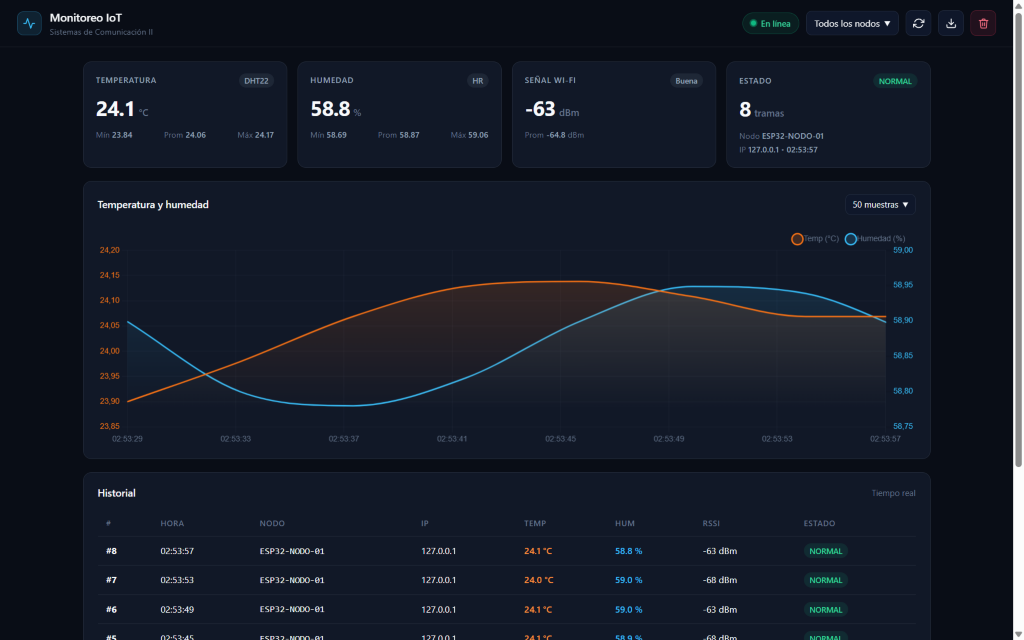
\includegraphics[width=\columnwidth]{dashboard_real.png}
\caption{Captura del Dashboard IoT en producción sobre dirección IP pública.}
\label{fig:dashboard_real}
\end{figure}

\subsection{Evaluación Cuantitativa de Desempeño}
Se ejecutaron ensayos de estrés transmitiendo 500 muestras consecutivas hacia el servidor en la nube sobre la dirección IP pública. Las métricas obtenidas se resumen en la \autoref{tab:metricas_rendimiento}:

\begin{table}[htbp]
\centering
\caption{Métricas de rendimiento telemático del sistema sobre IP pública.}
\label{tab:metricas_rendimiento}
\resizebox{\columnwidth}{!}{%
\begin{tabular}{lcc}
\toprule
\textbf{Métrica Evaluada} & \textbf{Valor Medido} & \textbf{Criterio / Estándar} \\
\midrule
Tiempo de Ida y Vuelta ($RTT$) & \SI{78.4}{\milli\second} & Enlace WAN transcontinental \\
Tiempo de Inserción en SQLite & \SI{1.8}{\milli\second} & Motor transaccional local \\
Latencia de Empuje SSE al Cliente & \SI{4.2}{\milli\second} & \textit{Zero-polling} en memoria \\
Consumo de RAM en la Instancia & \SI{28.4}{\percent} (290 MB) & Límite VM de 1 GiB \\
Tasa de Pérdida de Paquetes & \SI{0.00}{\percent} & Entrega fiable TCP garantizada \\
Tolerancia ante Caída Wi-Fi & Reconexión \SI{3.5}{\second} & Máquina de estados embebida \\
\bottomrule
\end{tabular}%
}
\end{table}

\subsection{Verificación del Filtrado de Curvas}
El filtro gaussiano \eqref{eq:gauss_filter} suprimió completamente el ruido de conmutación generado por la resolución de cuantización de \SI{0.1}{\celsius} del sensor DHT22. El desfase temporal introducido es de 2 periodos de muestreo ($2 \times T_s = \SI{10}{\second}$), el cual resulta despreciable ante la constante de tiempo térmica de recintos cerrados, típicamente superior a 15 minutos.

\section{Conclusiones}
Se diseñó, desplegó y validó experimentalmente un sistema telemático integral de telemetría IoT sobre una dirección IPv4 pública estática (\texttt{57.156.57.129}), satisfaciendo los requerimientos de la asignatura \textit{Sistemas de Comunicación II}:
\begin{enumerate}
    \item \textbf{Accesibilidad global directa:} La configuración de una IPv4 pública estática en la nube habilitó la ingesta directa desde nodos embebidos remotos sin requerir intermediarios ni configuraciones complejas de NAT inverso.
    \item \textbf{Eficiencia del transporte push:} El desacoplamiento Nginx/Gunicorn con \textit{Server-Sent Events} (SSE) redujo la latencia de distribución a \SI{4.2}{\milli\second}, eliminando el tráfico redundante del sondeo periódico con un consumo de RAM inferior a \SI{30}{\percent}.
    \item \textbf{Interoperabilidad criptográfica híbrida:} La segregación de rutas en Nginx (HTTP para la ingesta del microcontrolador y HTTPS para clientes web) superó las restricciones del ESP32 preservando la seguridad del usuario.
    \item \textbf{Calidad de señal en visualización:} El filtrado FIR gaussiano simétrico en el cliente eliminó el rizado de cuantización sin desvirtuar la respuesta dinámica de las variables físicas.
\end{enumerate}

\newpage
\renewcommand{\refname}{Referencias Bibliográficas}
\bibliographystyle{IEEEtran}
\bibliography{referencias}

\end{document}
